\documentclass[11pt]{article}
\usepackage{amsmath, amssymb, physics}
\usepackage{tikz}
\usetikzlibrary{decorations.pathmorphing, decorations.markings, arrows.meta}
\tikzset{->-/.style={decoration={markings, mark=at position #1 with {\arrow{Latex}}}, postaction={decorate}}}
\usepackage{pgfplots}
\pgfplotsset{compat=1.18}
\usepackage[margin=2.2cm]{geometry}
\usepackage{siunitx}
\usepackage{xcolor}
\usepackage{enumitem}
\usepackage{tcolorbox}
\usepackage{hyperref}
\hypersetup{colorlinks=true, linkcolor=blue}
\usepackage{array}

\newtcolorbox{question}{colback=blue!5!white, colframe=blue!60!black,
  fonttitle=\bfseries, before skip=8pt, after skip=8pt, boxsep=4pt,
  left=6pt, right=6pt, top=4pt, bottom=4pt,
  coltext=blue!50!black}

\newcommand{\Q}[1]{\begin{question}#1\end{question}}
\newcommand{\fphoton}[2]{\draw[decorate, decoration={snake, amplitude=0.6mm, segment length=2mm}] (#1) -- (#2);}
\newcommand{\fm}{\,\mathrm{fm}}
\newcommand{\MeV}{\,\mathrm{MeV}}
\newcommand{\GeV}{\,\mathrm{GeV}}

\title{B4 Subatomic Physics --- Problem Sheet 5 Solutions}
\author{}
\date{}

\begin{document}
\maketitle

\noindent\textit{SEMF: $B(Z,A)=a_V A-a_S A^{2/3}-a_C Z^{2}/A^{1/3}-a_A(A-2Z)^{2}/A+\delta(Z,A)$ with $a_V=15.56$, $a_S=17.23$, $a_C=0.697$, $a_A=23.285\MeV$; $\delta=\mp 12/A^{1/2}\MeV$ for odd-odd / even-even, 0 for odd-$A$. $r=r_0 A^{1/3}$, $r_0=1.2\fm$.}

%==================================================================
\section*{5.1 \quad Fermi theory of $\beta$ decay}

\Q{$\Gamma(p)\,dp=G_F^{2}/(2\pi^{3}\hbar^{7}c^{3})\cdot p^{2}(Q-E)^{2}\,dp$.\\
(a) Sketch the spectrum and justify form.\\
(b) Show $\Gamma\propto Q^{5}$ (Sargent's rule) for $Q\gg m_e c^{2}$.\\
(c) Allowed spin states of $e\bar\nu$ system.\\
(d) Three decays: do their relative rates follow Sargent? Explain.}

\paragraph{(a) Spectrum sketch.} Phase-space factors:
\begin{itemize}[itemsep=1pt]
\item $p^{2}\,dp$: density of final-state momenta for the electron.
\item $(Q-E)^{2}$: $\propto p_\nu^{2}$ for the neutrino in the massless limit.
\end{itemize}
The matrix element $|M|^{2}\propto G_F^{2}$ is taken constant (allowed transitions; no leptonic momentum dependence in the matrix element).

Key assumptions: (i) $V$-$A$ four-fermion contact interaction (Fermi); (ii) lepton wavefunctions are plane waves, so the matrix element is $E$-independent; (iii) $m_\nu=0$; (iv) recoil of the daughter nucleus is neglected; (v) Coulomb distortion of the outgoing electron in the nuclear field (Fermi function $F(Z,E)$) is set to unity.

\begin{center}
\begin{tikzpicture}
\begin{axis}[width=10cm,height=5cm,
   xlabel={$E$ (kinetic energy of $e^-$)},
   ylabel={$\Gamma(E)$},
   xmin=0,xmax=1.0,ymin=0,ymax=0.5,
   xtick={0,1},xticklabels={0,$Q$},
   ytick=\empty]
\addplot[domain=0.001:0.999, samples=100, blue, thick] {sqrt(x*(x+0.05))*(1-x)^2*(x+0.025)};
\end{axis}
\end{tikzpicture}
\end{center}
The spectrum vanishes at $E=0$ (as $p^{2}$) and at $E=Q$ (as $(Q-E)^{2}$), peaks somewhere around $E\sim Q/3$.

\paragraph{(b)} Use $E^{2}=p^{2}c^{2}+m_e^{2}c^{4}$ in the relativistic limit $E\simeq pc$:
\[
\Gamma=\frac{G_F^{2}}{2\pi^{3}\hbar^{7}c^{3}}\!\int_0^{Q/c}\!p^{2}(Q-pc)^{2}\,dp.
\]
Substitute $u=pc/Q\in[0,1]$, $dp=Q\,du/c$, $p^{2}=Q^{2}u^{2}/c^{2}$:
\[
\Gamma=\frac{G_F^{2}}{2\pi^{3}\hbar^{7}c^{3}}\cdot\frac{Q^{5}}{c^{3}}\!\int_0^{1}\!u^{2}(1-u)^{2}\,du
     =\frac{G_F^{2} Q^{5}}{60\pi^{3}\hbar^{7}c^{6}}.
\]
\[
\boxed{\;\Gamma\propto Q^{5}\quad\text{(Sargent's rule).}\;}
\]
\textbf{Numerical}: $\int_0^1 u^{2}(1-u)^{2}\,du=B(3,3)=2!\,2!/5!=1/30$, but combined with the prefactor $1/2$ this gives $1/60$. (Some texts write it with different overall constants; the $Q^{5}$ scaling is universal.)

\paragraph{(c) Spin states.} Two spin-$1/2$ leptons combine to total $S=0$ (singlet, antiparallel spins) or $S=1$ (triplet, parallel spins).
\begin{itemize}[itemsep=1pt]
\item $S=0$: \textbf{Fermi transition}. $\Delta J=0$, no parity change.
\item $S=1$: \textbf{Gamow--Teller transition}. $\Delta J=0,\pm 1$ (no $0\to 0$), no parity change.
\end{itemize}
For both, "allowed" implies the leptons carry no orbital angular momentum, $L_{e\nu}=0$.

\paragraph{(d) Sargent test.}
\begin{center}
\begin{tabular}{@{}lccccc@{}}\hline
Decay & $J_i\to J_f$ & Type & $Q$ [MeV] & $t_{1/2}$ [s] & $\Gamma\,Q^{-5}$ relative\\\hline
$^{6}$He$\to{}^{6}$Li & $0^+\to 1^+$ & Gamow-Teller & 3.5 & 0.81 & ref\\
$^{3}$H$\to{}^{3}$He & $\tfrac12^+\to\tfrac12^+$ & F+GT & 0.018 & $4\times 10^{8}$ & ?\\
$^{10}$Be$\to{}^{10}$B & $0^+\to 3^+$ & forbidden & 0.55 & $5\times 10^{13}$ & ?\\\hline
\end{tabular}
\end{center}

Predict if Sargent holds: $\Gamma_i/\Gamma_j=(Q_i/Q_j)^{5}$.\\
Reference $^{6}$He: $\Gamma_0=\ln 2/0.81=0.856\,\mathrm{s^{-1}}$, $Q_0^{5}=3.5^{5}=525.2$.\\
$^{3}$H: $\Gamma_1=\ln 2/(4\times 10^{8})=1.73\times 10^{-9}\,\mathrm{s^{-1}}$, $Q_1^{5}=0.018^{5}=1.89\times 10^{-9}$.\\
Predicted by Sargent (relative to $^{6}$He): $\Gamma_1^\mathrm{pred}=0.856\cdot 1.89\times 10^{-9}/525.2=3.08\times 10^{-12}\,\mathrm{s^{-1}}$. Observed: $1.73\times 10^{-9}$. \textbf{Observed is $\sim 560\times$ faster} than Sargent predicts.

$^{10}$Be: $\Gamma_2=\ln 2/(5\times 10^{13})=1.39\times 10^{-14}\,\mathrm{s^{-1}}$, $Q_2^{5}=0.55^{5}=0.0503$. Predicted: $0.856\cdot 0.0503/525.2=8.20\times 10^{-5}\,\mathrm{s^{-1}}$. Observed $1.39\times 10^{-14}$. \textbf{Observed is $\sim 6\times 10^{9}$ times slower} than Sargent.

\textbf{Explanations:}
\begin{itemize}[itemsep=1pt]
\item $^{3}$H is "super-allowed" (mirror nuclei, near-perfect overlap of nuclear wavefunctions) — Sargent gives the correct \emph{scaling}, but $^{6}$He has a smaller-than-unity nuclear matrix element relative to a super-allowed transition. The $\sim 560$ enhancement in $^3$H is from a larger nuclear matrix element, not phase space.
\item $^{10}$Be$(0^+)\to{}^{10}$B$(3^+)$ requires $\Delta J=3$, which is \textbf{third-forbidden}: the leptons must carry off $L=2$ orbital angular momentum together with $S=1$. The matrix element is suppressed by a factor $\sim(p R/\hbar)^{2L}\sim 10^{-8}$, vastly slowing the decay.
\end{itemize}

The bottom line: Sargent's $Q^{5}$ scaling holds only when comparing transitions with similar nuclear matrix elements (same forbiddenness class).

%==================================================================
\section*{5.2 \quad Stability against $\beta$ decay}

\Q{(a) Use SEMF to predict the stable isobar with $A=181$.\\
(b) Stable nuclei tally: 177 e-e, 121 e-o, 8 o-o. (i) Explain graphically. (ii) Why is $^{76}$Ge actually unstable with $t_{1/2}=2\times 10^{21}$ yr?}

\paragraph{(a) $A=181$ (odd $A$).} Pairing $\delta=0$. Minimise SEMF mass $\Leftrightarrow$ maximise $B$:
\[
\frac{\partial B}{\partial Z}\Big|_A=-\frac{2 a_C Z}{A^{1/3}}+\frac{4 a_A(A-2Z)}{A}=0.
\]
\[
Z_*=\frac{A}{2}\cdot\frac{1}{1+a_C A^{2/3}/(4 a_A)}.
\]
With $A=181$: $A^{2/3}=181^{2/3}=31.93$. $a_C A^{2/3}/(4 a_A)=0.697\cdot 31.93/(4\cdot 23.285)=22.26/93.14=0.239$.
\[
Z_*=\frac{181}{2}\cdot\frac{1}{1.239}=90.5/1.239=73.07.
\]
Round to nearest integer: \textbf{$Z=73$}, which is \textbf{$^{181}_{\,73}$Ta} (tantalum). Observed: $^{181}$Ta is the unique stable isobar at $A=181$ \checkmark.

\paragraph{(b)(i) Mass parabolas.} Plot $M(A,Z)$ vs.\ $Z$ at fixed $A$. From the SEMF this is a parabola in $Z$ (Coulomb $Z^{2}$, asymmetry $(A-2Z)^{2}$). Pairing shifts the parabola.

\textbf{Odd $A$:} all isobars are odd-$A$, $\delta=0$. Single parabola; only one $Z$ at the bottom is stable; neighbours $\beta$-decay (one direction) and EC/$\beta^{+}$ (the other direction) toward it.

\textbf{Even $A$:} two parabolas, separated by $2|\delta|$. Even-even (lower) and odd-odd (upper). Stable nuclei sit on the lower (even-even) parabola; multiple even-even isobars can be stable because $\beta$-decay between them would require passing through the higher odd-odd parabola, which is energetically forbidden for some pairs.

\begin{center}
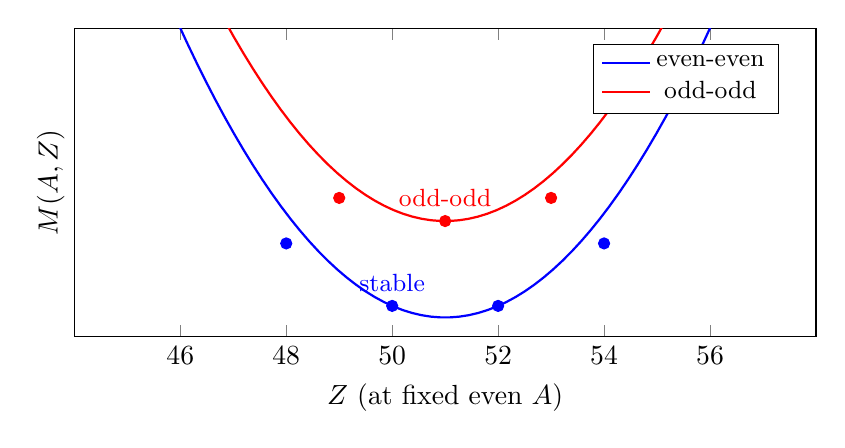
\begin{tikzpicture}
\begin{axis}[width=11cm,height=5.5cm,
   xlabel={$Z$ (at fixed even $A$)},ylabel={$M(A,Z)$},
   xmin=44,xmax=58,ymin=0,ymax=8,
   xtick={46,48,50,52,54,56},
   ytick=\empty,
   legend style={at={(0.95,0.95)},anchor=north east,font=\small}]
\addplot[thick,blue,domain=44:58,samples=80] {0.3*(x-51)^2+0.5};
\addlegendentry{even-even}
\addplot[thick,red,domain=44:58,samples=80] {0.3*(x-51)^2+3};
\addlegendentry{odd-odd}
\addplot[only marks,mark=*,blue] coordinates {(48,2.42) (50,0.8) (52,0.8) (54,2.42)};
\addplot[only marks,mark=*,red] coordinates {(49,3.6) (51,3.0) (53,3.6)};
\node[blue] at (axis cs:50,1.4) {\small stable};
\node[red] at (axis cs:51,3.6) {\small odd-odd};
\end{axis}
\end{tikzpicture}
\end{center}

For odd-odd isobars: only a few exceptions are stable ($^{2}$H, $^{6}$Li, $^{10}$B, $^{14}$N, $^{40}$K, $^{50}$V, $^{138}$La, $^{180}$Ta-m: 8 in total). They sit at the bottom of the upper parabola without an even-even neighbour energetically below them — but most odd-odd nuclei \emph{do} have such a neighbour and decay quickly.

\paragraph{(b)(ii) $^{76}$Ge ($Z=32, A=76$).} Even-even, $A=76$ parabola minimum. Naively SEMF says it is the bottom of its parabola and should be stable. Let me check the parabola at $A=76$:
$Z_*=A/2/(1+a_C A^{2/3}/(4a_A))$. $76^{2/3}=17.93$. $0.697\cdot 17.93/(4\cdot 23.285)=12.5/93.14=0.134$. $Z_*=38/1.134=33.5$. So the minimum is around $Z=33$ or 34 (even-even $Z$). Actually $^{76}_{34}$Se is the even-even isobar nearest the minimum. $^{76}_{32}$Ge is to the left and would naively want to $\beta^-$-decay to $^{76}_{33}$As (odd-odd), but the odd-odd parabola is \emph{higher} due to negative pairing $\delta$. So the single $\beta^-$ transition $^{76}$Ge $\to{}^{76}$As is energetically forbidden.

The only available decay is \textbf{double beta decay}: $^{76}$Ge $\to{}^{76}$Se + 2$e^-$ + 2$\bar\nu_e$. This is a second-order weak process with $G_F^{4}$ rate, hence the enormous half-life $\sim 10^{21}$ yr. (Indeed, $^{76}$Ge is a major target nucleus for searches for \emph{neutrinoless} double beta decay --- GERDA, LEGEND --- because both modes are observable.)

%==================================================================
\section*{5.3 \quad Fission reactors}

\Q{(a) Why is $^{235}$U fissile and $^{238}$U not? Role of moderator; pros/cons of choices; why not homogeneous?\\
(b) Asymmetric fragments ($A\sim 93,140$): where on stability valley? SEMF $Z_*$ for these. Energy released, fuel mass for 1 GW reactor.\\
(c) How are $^{233}$U and $^{239}$Pu produced from U/Th feed?}

\paragraph{(a) Fissility of $^{235}$U vs $^{238}$U.} 

$^{235}$U has $A=235$ (odd), so adding a neutron gives $^{236}$U with $A=236$ (even). Pairing energy $\delta(Z,A)=+12/\sqrt{A}\MeV\simeq +0.78\MeV$ for the resulting even-even nucleus enhances the binding by $\sim 1.6\MeV$ compared to the odd-$A$ case. The neutron separation energy in $^{236}$U:
\[
S_n=B(^{236}\text{U})-B(^{235}\text{U})\simeq 6.5\MeV.
\]
For $^{238}$U + $n\to{}^{239}$U (odd-$A$, no pairing bonus): $S_n\simeq 4.8\MeV$.

The fission barrier for both is $\sim 6\MeV$. Thermal neutrons (kinetic energy $\sim 0.025$ eV) bring negligible kinetic energy, so the only energy available is $S_n$:
\begin{itemize}[itemsep=1pt]
\item $^{235}$U: $S_n=6.5\MeV>$ barrier $\Rightarrow$ thermal neutrons induce fission. \textbf{Fissile.}
\item $^{238}$U: $S_n=4.8\MeV<$ barrier $\Rightarrow$ requires \emph{fast} neutrons ($E\gtrsim 1\MeV$). \textbf{Fissionable but not fissile.}
\end{itemize}

\textbf{Moderator role.} Fission neutrons are emitted at $\sim 2\MeV$. To exploit the high $^{235}$U thermal-neutron fission cross section ($\sigma_f\sim 580$ b at thermal vs.\ $\sim 1$ b at fast), neutrons must be slowed to thermal energies via elastic scattering on light nuclei (which absorb a maximum fraction of the neutron's energy in a head-on collision: $\Delta E/E=4 m_n M/(m_n+M)^{2}$).

\textbf{Choices:}
\begin{itemize}[itemsep=1pt]
\item \textbf{Light water $^{1}$H}: best moderator (large $\Delta E/E\simeq 1$); but absorbs neutrons via $n+p\to d+\gamma$ ($\sigma\sim 0.33$ b), so requires enriched $^{235}$U ($\sim 3\%$).
\item \textbf{Heavy water $^{2}$H (D$_2$O)}: still excellent slowing-down, with much smaller absorption ($\sigma_a\sim 0.5\,\mathrm{mb}$). Allows natural-uranium reactors (CANDU). Expensive to produce.
\item \textbf{Graphite ($^{12}$C)}: low absorption, decent moderation. Used in early reactors and RBMK; less compact, fire risk (Chernobyl).
\item \textbf{Beryllium}: good but expensive and toxic.
\end{itemize}

\textbf{Why not homogeneous fuel + moderator mix?} Because the resonance absorption cross sections of $^{238}$U at intermediate energies (1 eV–1 keV) are huge (peaks $\sim 10^{4}$ b). If neutrons are slowing through these resonance energies \emph{within} the fuel, they are captured by $^{238}$U non-productively. By keeping fuel in pellets/rods and the moderator in between, neutrons traverse most of the moderation outside the fuel, where they cannot be captured by $^{238}$U, and only re-enter the fuel at thermal energies where $^{235}$U fission cross section dominates. This is \textbf{spatial self-shielding}.

\paragraph{(b) Asymmetric fragments $A=93,140$.}

\textbf{Predicted stable $Z$ from SEMF:}
$A=93$: $93^{2/3}=20.78$. $a_C A^{2/3}/(4a_A)=0.697\cdot 20.78/93.14=0.156$. $Z_*=46.5/1.156=40.2$ $\Rightarrow Z=40$ ($^{93}$Zr).\\
$A=140$: $140^{2/3}=27.40$. Factor: $0.697\cdot 27.40/93.14=0.205$. $Z_*=70/1.205=58.1$ $\Rightarrow Z=58$ ($^{140}$Ce).

\textbf{Where are the actual fission products?} The original $^{236}$U has $N/Z=144/92=1.565$. If it splits into two fragments preserving this ratio: a fragment with $A=93$ would have $Z\simeq 93/2.565=36$ ($^{93}$Kr), and $A=140$ would have $Z\simeq 140/2.565=55$ ($^{140}$Cs). These are \textbf{neutron-rich} compared to the stability line ($Z_*=40$ and 58 respectively).

The fragments $\beta^-$-decay back toward stability through chains of $\beta^-$ emissions:
\[
^{93}\mathrm{Kr}\to{}^{93}\mathrm{Rb}\to{}^{93}\mathrm{Sr}\to{}^{93}\mathrm{Y}\to{}^{93}\mathrm{Zr}\;(\text{stable}).
\]
Some intermediate states emit \textbf{delayed neutrons}, which are crucial for reactor control.

\textbf{Energy released.} From the SEMF or from a binding-energy table: the total kinetic energy released per fission is
\[
Q_\mathrm{fission}\simeq B(^{93}\text{Zr})+B(^{140}\text{Ce})-B(^{236}\text{U})\simeq 200\MeV.
\]
(More precisely $\sim 215\MeV$ if including $\beta$ + $\gamma$ from delayed activity; "prompt" $\sim 175$ MeV.)

\textbf{Mass of $^{235}$U per second for 1 GW.}
\[
\frac{dN}{dt}=\frac{P}{Q_\mathrm{fission}}=\frac{10^{9}\,\mathrm{W}}{200\MeV\cdot 1.602\times 10^{-13}\,\mathrm{J/MeV}}=\frac{10^{9}}{3.20\times 10^{-11}}=3.12\times 10^{19}\,\mathrm{fissions/s}.
\]
\[
\frac{dm}{dt}=\frac{dN}{dt}\cdot\frac{M}{N_A}=3.12\times 10^{19}\cdot\frac{0.235}{6.022\times 10^{23}}=\boxed{\,1.22\times 10^{-5}\,\mathrm{kg/s}\simeq 1\,\mathrm{kg/day}.\,}
\]
(For a thermal reactor with electrical efficiency $\sim 33\%$, a 1 GW$_e$ reactor consumes $\sim 3$ kg/day of $^{235}$U.)

\paragraph{(c) Breeding fissile fuel.}

\textbf{$^{239}$Pu from $^{238}$U:}
\[
n+{}^{238}\mathrm{U}\to{}^{239}\mathrm{U}\xrightarrow{\beta^-,\,t_{1/2}=23.5\,\mathrm{min}}{}^{239}\mathrm{Np}\xrightarrow{\beta^-,\,t_{1/2}=2.36\,\mathrm{d}}{}^{239}\mathrm{Pu}.
\]

\textbf{$^{233}$U from $^{232}$Th:}
\[
n+{}^{232}\mathrm{Th}\to{}^{233}\mathrm{Th}\xrightarrow{\beta^-,\,22\,\mathrm{min}}{}^{233}\mathrm{Pa}\xrightarrow{\beta^-,\,27\,\mathrm{d}}{}^{233}\mathrm{U}.
\]

Both feeds are non-fissile but \emph{fertile}: they capture a neutron and after two $\beta^-$ steps yield a fissile actinide. \textbf{Breeder reactors} are designed to produce more fissile material than they consume by maintaining a high fast-neutron flux that exceeds the breeding threshold ($\eta>2$, the number of fission neutrons per absorbed neutron must exceed 2 to sustain criticality plus breed one new fissile atom).

%==================================================================
\section*{5.4 \quad Natural fission reactors}

\Q{(a) From the present $^{235}$U/$^{238}$U ratio of $7.2\times 10^{-3}$, with mean lives $1.03\times 10^{9}$ and $6.49\times 10^{9}$ yr, find the time since equal production.\\
(b) Oklo: ratio is $5\times 10^{-3}$, $\sim 10^{5}$ kg ore, fission $\sim 2$ Gyr ago lasting $\sim 10^{6}$ yr. Energy and mean power.\\
(c) Other evidence; why none today?}

\paragraph{(a) Time since equal abundance.}
\[
\frac{N_{235}(t)}{N_{238}(t)}=\frac{N_{235}(0)e^{-t/\tau_{235}}}{N_{238}(0)e^{-t/\tau_{238}}}=e^{-t(1/\tau_{235}-1/\tau_{238})}.
\]
Setting $N_{235}(0)=N_{238}(0)$:
\[
7.2\times 10^{-3}=e^{-t(1/\tau_{235}-1/\tau_{238})},
\]
\[
1/\tau_{235}-1/\tau_{238}=(1/1.03-1/6.49)\times 10^{-9}\,\mathrm{yr^{-1}}=(0.971-0.154)\times 10^{-9}=8.17\times 10^{-10}\,\mathrm{yr^{-1}}.
\]
\[
t=\frac{-\ln(7.2\times 10^{-3})}{8.17\times 10^{-10}}\,\mathrm{yr}=\frac{4.93}{8.17\times 10^{-10}}=\boxed{\,6.0\times 10^{9}\,\mathrm{yr}.\,}
\]
This is older than the solar system ($4.6$ Gyr); that's fine because the assumption "equal abundance at production" refers to the time of \emph{nucleosynthesis} (in supernovae predating the solar system).

\paragraph{(b) Oklo energy and power.}

\textbf{Mass of $^{235}$U fissioned.} $2$ Gyr ago, the natural-uranium $^{235}$U fraction was higher. Recompute it: $r(t_\mathrm{Oklo})=r_\mathrm{now}\cdot e^{(t_\mathrm{Oklo})(1/\tau_{235}-1/\tau_{238})}=7.2\times 10^{-3}\cdot e^{2\times 10^{9}\cdot 8.17\times 10^{-10}}=7.2\times 10^{-3}\cdot e^{1.634}=7.2\times 10^{-3}\cdot 5.12=3.69\times 10^{-2}$.

So at Oklo time, natural U was $\sim 3.7\%$ $^{235}$U — \emph{enrichment level of modern PWR fuel}. That's why a natural reactor was possible.

The reduction from $3.7\%$ to $0.5\%$ (the depleted Oklo $^{235}$U fraction quoted: $5\times 10^{-3}$ relative to $^{238}$U $\Rightarrow$ $5\times 10^{-3}/(1+5\times 10^{-3})\simeq 0.5\%$) means the "missing" fraction has been fissioned. Actually the comparison is between $r=3.69\times 10^{-2}$ and $r=5\times 10^{-3}$; the change in the $^{235}$U/$^{238}$U ratio reflects both decay and fission depletion. The decay alone over 2 Gyr would have brought it from 3.7\% to $0.72\%$. The Oklo deposit is at $0.5\%$, so the fission depletion is the difference.

Fraction of $^{235}$U fissioned $\simeq(0.72-0.5)/0.72=0.31$, of about $0.72\%$ of total mass at Oklo time, on a $10^{5}$ kg deposit:
\[
m_\mathrm{fissioned}\simeq 0.0072\cdot 0.31\cdot 10^{5}\,\mathrm{kg}\simeq 220\,\mathrm{kg}.
\]
At $\sim 200$ MeV per fission and $N_A/0.235$ fissions per kg of $^{235}$U:
\[
N_\mathrm{fiss}=220\,\mathrm{kg}\cdot\frac{6.022\times 10^{23}}{0.235}=5.64\times 10^{26},
\]
\[
E_\mathrm{tot}=5.64\times 10^{26}\cdot 200\MeV=1.13\times 10^{29}\MeV=1.81\times 10^{16}\,\mathrm{J}=\boxed{\,18\,\mathrm{PJ}.\,}
\]

\textbf{Mean power} over $10^{6}$ yr $=3.15\times 10^{13}$ s:
\[
\langle P\rangle=\frac{1.81\times 10^{16}\,\mathrm{J}}{3.15\times 10^{13}\,\mathrm{s}}=\boxed{\,580\,\mathrm{W}.\,}
\]
(Modest! Only a few hundred watts on average. Local geological and chemical evidence suggests it operated in pulses — water boiling out, criticality lost, water returning, criticality restored — like a self-regulating geyser of fission, with peak power probably much higher.)

\paragraph{(c) Other evidence and why none today.}

\textbf{Evidence:}
\begin{itemize}[itemsep=1pt]
\item Anomalous isotopic composition of fission products: $^{142}$Nd, $^{143}$Nd, $^{145}$Nd, $^{146}$Nd ratios deviate from natural ones, matching fission yields.
\item Depleted-in-$^{235}$U uranium ore in specific zones (the chemical signature).
\item Unusual abundances of fission-derived stable nuclides (Ru, Rh isotopes).
\item Trace plutonium and $^{99}$Tc (now decayed; daughter products preserved).
\end{itemize}

\textbf{Why none today:}
\begin{itemize}[itemsep=1pt]
\item Natural $^{235}$U abundance is now only 0.72\% — too low to sustain criticality with light-water moderation in any natural geological setting. Going below $\sim 1\%$ enrichment is fatal.
\item No ongoing tectonic processes are concentrating uranium with sufficient water, geometry, and absence of neutron poisons.
\end{itemize}

%==================================================================
\section*{5.5 \quad Fusion}

\Q{(a) $\sigma=(S/E)e^{-C/\sqrt E}$. Justify; show $C=Z_1 Z_2\sqrt{A_1 A_2/(A_1+A_2)}\cdot 31.4\,\mathrm{(keV)}^{1/2}$. Gamow peak position and height $\propto\exp[-1.89(C^{2}/k_B T)^{1/3}]$.\\
(b) $pp$ chain in solar core: $T=10^{7}$ K $\Rightarrow$ 1 mW/kg. Predict at $T=10^{6}$ and $10^{8}$ K.\\
(c) Ratio $^{2}$H+$^{3}$H to $^{2}$H+$^{3}$He at $T=2\times 10^{8}$ K.\\
(d) Coulomb barrier and fusion energy release for $^{10}$B+$^{10}$B, $^{12}$C+$^{12}$C, $^{16}$O+$^{16}$O.}

\paragraph{(a) Form and $C$.} Cross section:
\begin{itemize}[itemsep=1pt]
\item $1/E$ from de Broglie wavelength squared: $\pi\lambda^{2}\propto 1/p^{2}\propto 1/E$.
\item $e^{-C/\sqrt E}$ Gamow factor for tunnelling through Coulomb barrier (analogous to $\alpha$-decay Sec.\ 4.7 but with sub-barrier kinematics; particle has reduced mass $\mu=m_1 m_2/(m_1+m_2)$):
\end{itemize}
\[
C=\frac{2\pi Z_1 Z_2 e^{2}\sqrt{2\mu}}{4\pi\epsilon_{0}\hbar\sqrt{1}}=\frac{2\pi Z_1 Z_2 e^{2}}{4\pi\epsilon_{0}\hbar c}\cdot\sqrt{2\mu c^{2}}.
\]
With $\mu c^{2}=A_1 A_2/(A_1+A_2)\cdot u c^{2}$, $u c^{2}=931.5\MeV$:
\[
C=2\pi\alpha Z_1 Z_2\sqrt{2 A_1 A_2/(A_1+A_2)\cdot 931500}\,\mathrm{(keV)}^{1/2}=Z_1 Z_2\sqrt{A_1 A_2/(A_1+A_2)}\cdot 31.4\,\mathrm{(keV)^{1/2}}.
\]
\checkmark

\textbf{Gamow peak.} Total fusion rate from a Maxwell--Boltzmann gas at temperature $T$:
\[
R\propto\!\int_0^\infty\!E\, e^{-E/k_B T}\sigma(E)\,dE=S\!\int_0^\infty\!\exp\!\left[-E/k_B T-C/\sqrt E\right]\,dE.
\]
The exponent has a maximum where $\frac{d}{dE}[-E/k_B T-C/\sqrt E]=-1/k_B T+C/(2 E^{3/2})=0$:
\[
E_G=\!\left(\frac{C k_B T}{2}\right)^{2/3}.
\]
Substituting back, the exponent at the peak:
\[
-\frac{E_G}{k_B T}-\frac{C}{\sqrt{E_G}}=-3\frac{E_G}{k_B T}\!\bigg|_{(\text{algebra})}=-3\!\left(\frac{C^{2}}{4 k_B T}\right)^{1/3}\!.
\]
Wait, let me redo more carefully. Let $x=E^{1/2}$, so $f(x)=-x^{2}/(k_B T)-C/x$. Stationary: $-2x/(k_B T)+C/x^{2}=0\Rightarrow x^{3}=C k_B T/2$, i.e.\ $x_*=(C k_B T/2)^{1/3}$. Then $E_G=x_*^{2}=(C k_B T/2)^{2/3}$. The exponent at peak: $-x_*^{2}/k_B T-C/x_*=-x_*^{2}/k_B T-2 x_*^{2}/k_B T=-3 x_*^{2}/k_B T=-3(C^{2}/4)^{1/3}/(k_B T)^{1/3}=-3(C^{2}/[4 k_B T])^{1/3}$.

Numerically, $3/4^{1/3}=3/1.587=1.890$. So
\[
\boxed{\;R\propto\exp\!\left[-1.89\!\left(\frac{C^{2}}{k_B T}\right)^{1/3}\right]\,.\;}
\]

\paragraph{(b) Sun: $T$ scaling of $pp$ rate.} For $p+p$, $Z_1=Z_2=1$, $A_1=A_2=1$, so $C=1\cdot\sqrt{1/2}\cdot 31.4=22.2\,\mathrm{keV}^{1/2}$, $C^{2}=494\,\mathrm{keV}=494\times 10^{3}$ eV.\\
At $T_0=10^{7}$ K: $k_B T_0=1.381\times 10^{-23}\cdot 10^{7}=1.381\times 10^{-16}$ J $=863$ eV. So $C^{2}/(k_B T_0)=494000/863=572$, $\Rightarrow$ argument of exp: $-1.89\cdot(572)^{1/3}=-1.89\cdot 8.30=-15.69$, $e^{-15.69}=1.53\times 10^{-7}$. The "1 mW/kg" at $T_0$ corresponds to this Gamow exponent.

\textbf{At $T_1=10^{6}$ K:} $C^{2}/k_B T_1=10\cdot 572=5720$. $1.89\cdot 5720^{1/3}=1.89\cdot 17.88=33.79$. $e^{-33.79}=2.13\times 10^{-15}$. Ratio:
\[
\frac{P(T_1)}{P(T_0)}=\frac{2.13\times 10^{-15}}{1.53\times 10^{-7}}=1.4\times 10^{-8}.
\]
\textbf{Power at $T=10^{6}$ K: $\sim 1.4\times 10^{-11}\,\mathrm{W/kg}$.}

\textbf{At $T_2=10^{8}$ K:} $C^{2}/k_B T_2=572/10=57.2$. $1.89\cdot 57.2^{1/3}=1.89\cdot 3.85=7.28$. $e^{-7.28}=6.86\times 10^{-4}$. Ratio:
\[
\frac{P(T_2)}{P(T_0)}=\frac{6.86\times 10^{-4}}{1.53\times 10^{-7}}=4.5\times 10^{3}.
\]
\textbf{Power at $T=10^{8}$ K: $\sim 4.5\,\mathrm{W/kg}$.} (Note: at this temperature one should also include the temperature dependence of the prefactor and re-evaluate $S$, but the Gamow exponential dominates.)

\paragraph{(c) $^{2}$H+$^{3}$H vs.\ $^{2}$H+$^{3}$He at $T=2\times 10^{8}$ K.}
Both have $Z_1=1$, but $Z_2$ differs:
\begin{itemize}[itemsep=0pt]
\item DT: $Z_2=1$, $\mu=2\cdot 3/(2+3)=1.2$. $C_\mathrm{DT}=1\cdot 1\cdot\sqrt{1.2}\cdot 31.4=34.4\,\mathrm{keV}^{1/2}$.
\item D+$^{3}$He: $Z_2=2$, $\mu=1.2$. $C_\mathrm{DHe}=1\cdot 2\cdot\sqrt{1.2}\cdot 31.4=68.8\,\mathrm{keV}^{1/2}$.
\end{itemize}
$k_B T=2\times 10^{8}\cdot 8.617\times 10^{-5}=17.2$ keV. $C^{2}/k_B T$:
\[
\mathrm{DT}: 34.4^{2}/17.2=1183/17.2=68.8.
\]
\[
\mathrm{DHe}: 68.8^{2}/17.2=4734/17.2=275.2.
\]
Gamow exponents: $-1.89\cdot 68.8^{1/3}=-1.89\cdot 4.10=-7.75$. $-1.89\cdot 275.2^{1/3}=-1.89\cdot 6.51=-12.30$. Ratio of rates:
\[
\frac{R(\mathrm{DT})}{R(\mathrm{DHe})}=e^{-7.75-(-12.30)}=e^{4.55}=\boxed{\,95.\,}
\]
DT is favoured by about a factor of 100, despite both having the same available energy --- this is why DT is the chosen fusion reaction for ITER and DEMO.

\paragraph{(d) Coulomb barriers and energies for boron, carbon, oxygen burning.}

Coulomb barrier height: $V_C=Z_1 Z_2 e^{2}/(4\pi\epsilon_{0}r)$ at contact $r=r_0(A_1^{1/3}+A_2^{1/3})$:
\begin{center}
\begin{tabular}{@{}lcccc@{}}\hline
Reaction & $Z_1=Z_2$ & $r$ [fm] & $V_C$ [MeV] & $T$ at $V_C$ [K]\\\hline
$^{10}$B+$^{10}$B & 5 & $1.2\cdot 2\cdot 10^{1/3}=5.17$ & $25\cdot 1.44/5.17=6.96$ & $8.1\times 10^{10}$\\
$^{12}$C+$^{12}$C & 6 & $1.2\cdot 2\cdot 12^{1/3}=5.50$ & $36\cdot 1.44/5.50=9.42$ & $1.1\times 10^{11}$\\
$^{16}$O+$^{16}$O & 8 & $1.2\cdot 2\cdot 16^{1/3}=6.05$ & $64\cdot 1.44/6.05=15.23$ & $1.8\times 10^{11}$\\\hline
\end{tabular}
\end{center}

(The Gamow peak energy at relevant astrophysical temperatures is much smaller than $V_C$; tunnelling makes fusion possible at $T\sim 5\times 10^{8}$ K for C burning.)

\textbf{Energy release per fusion} (requires choosing a reaction channel; common ones):
\begin{itemize}[itemsep=1pt]
\item $^{12}$C+$^{12}$C: $\to{}^{20}$Ne+$\alpha$ ($Q=4.62\MeV$) or $\to{}^{23}$Mg+n ($-2.6\MeV$, endothermic) or $\to{}^{23}$Na+p ($Q=2.24\MeV$).
\item $^{16}$O+$^{16}$O: $\to{}^{28}$Si+$\alpha$ ($Q=9.59\MeV$), $\to{}^{31}$P+p ($7.68\MeV$), $\to{}^{31}$S+n ($1.45\MeV$).
\item $^{10}$B+$^{10}$B: $\to{}^{20}$Ne+? various exothermic channels of order $\sim 10\MeV$.
\end{itemize}
A clean estimate: from binding-energy difference $(2 B_\mathrm{reactant})-B_\mathrm{product}$. For $^{12}$C+$^{12}$C $\to{}^{24}$Mg: $B(^{24}\mathrm{Mg})=198.26$, $2 B(^{12}\mathrm{C})=2\cdot 92.16=184.32$; $Q=13.93\MeV$.

%==================================================================
\section*{5.6 \quad Resonances and compound nuclei}

\Q{$n+A\to B+\gamma$ via short-lived compound nucleus, $\Gamma_n$ proportional to neutron transition rate, $\Gamma$ independent of $E_n$.\\
(a) Show $\Gamma_n\propto p$, hence $\sigma\propto 1/v$ at low $E$.\\
(b) $^{113}$Cd capture data: extract $E_R$, $\Gamma$, $\Gamma_n(E_R)$, $\sigma_\mathrm{el}^\mathrm{max}$.\\
(c) Implication of narrow resonance dominantly decaying via $\gamma$.}

\paragraph{(a) Low-energy form.}
Density of states for the incoming neutron in a box of volume $V$:
\[
\frac{dn}{dE}=\frac{V}{(2\pi)^{3}}\cdot 4\pi p^{2}\cdot\frac{dp}{dE}=\frac{V p^{2}}{2\pi^{2}\hbar^{3}}\cdot\frac{dp}{dE}=\frac{V p m}{2\pi^{2}\hbar^{3}}.
\]
But the partial width comes from the matrix element times the $\nu$\textit{outgoing} density of states. For the entrance neutron channel, $\Gamma_n$ is the rate at which the compound nucleus can re-emit a neutron, which by Fermi's golden rule is $\propto p$:
\[
\Gamma_n(E)\propto p(E)\propto\sqrt E.
\]
Now apply Breit--Wigner with $\Gamma\sim$ const and $\Gamma_\gamma\sim$ const (photon emission rate is set by nuclear electromagnetic structure, independent of incoming neutron):
\[
\sigma_{n\gamma}\sim\frac{\pi}{k^{2}}\frac{\Gamma_n\Gamma_\gamma}{(E_R-E)^{2}+\Gamma^{2}/4}.
\]
At $E\ll E_R$: $\pi/k^{2}\propto 1/E$. $\Gamma_n\propto\sqrt E$. So:
\[
\sigma\propto\frac{1}{E}\cdot\sqrt E\cdot\frac{1}{(E_R-E)^{2}+\Gamma^{2}/4}\xrightarrow{E\ll E_R}\frac{1}{\sqrt E}=\frac{1}{v}.
\]
\[
\boxed{\;\sigma_{n\gamma}\propto\frac{1}{v}\quad\text{at low }E.\;}
\]

\paragraph{(b) Extracting $E_R,\Gamma,\Gamma_n$ from $^{113}$Cd data.}

The $1/v$ contribution dominates at very low $E$. Plot $\sigma\sqrt E$ to remove this trivial factor and reveal the resonance:

\begin{center}
\begin{tabular}{@{}cccc@{}}\hline
$E$ [eV] & $\sigma$ [b] & $\sqrt E$ & $\sigma\sqrt E$\\\hline
0.01 & 3250 & 0.100 & 325\\
0.02 & 2500 & 0.141 & 354\\
0.03 & 2300 & 0.173 & 398\\
0.05 & 2400 & 0.224 & 537\\
0.08 & 2800 & 0.283 & 792\\
0.10 & 3400 & 0.316 & 1075\\
0.15 & 6800 & 0.387 & 2634\\
0.20 & 6000 & 0.447 & 2683\\
0.25 & 2400 & 0.500 & 1200\\
0.30 & 1100 & 0.548 & 603\\
0.40 & 320 & 0.632 & 202\\
0.50 & 140 & 0.707 & 99\\\hline
\end{tabular}
\end{center}

\begin{center}
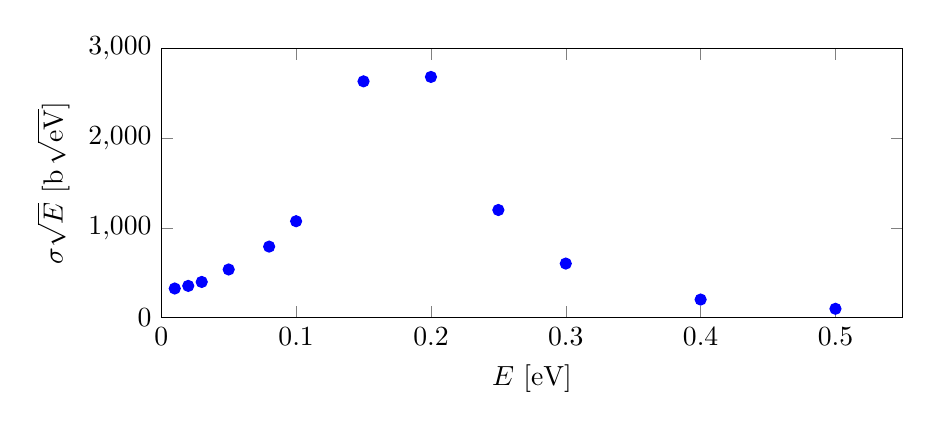
\begin{tikzpicture}
\begin{axis}[width=11cm,height=5cm,
   xlabel={$E$ [eV]},ylabel={$\sigma\sqrt E$ [b$\,\sqrt{\mathrm{eV}}$]},
   xmin=0,xmax=0.55,ymin=0,ymax=3000]
\addplot[only marks, mark=*, blue] coordinates {
  (0.01,325) (0.02,354) (0.03,398) (0.05,537) (0.08,792)
  (0.10,1075) (0.15,2634) (0.20,2683) (0.25,1200)
  (0.30,603) (0.40,202) (0.50,99)};
\end{axis}
\end{tikzpicture}
\end{center}

The peak in $\sigma\sqrt E$ is at $E\simeq 0.18$ eV (between 0.15 and 0.20). Interpolating, \textbf{$E_R\simeq 0.18$ eV}.

The peak value $\sigma_\mathrm{max}=7750\pm 150$ b at $E_R$. From the formula
\[
\sigma_{n\gamma}^\mathrm{peak}=\frac{4\pi g}{k^{2}_R}\frac{\Gamma_n\Gamma_\gamma}{\Gamma^{2}}\quad\text{with }g=(2J_R+1)/[(2s_n+1)(2J_A+1)]=3/[2\cdot 2]=3/4.
\]
Half-max occurs at $E_R\pm\Gamma/2$. From the data, the FWHM of the $\sigma\sqrt E$ peak is roughly between $E\simeq 0.10$ eV (1075) and $E\simeq 0.30$ eV (603), with peak $\sim 2683$. Half-max $\simeq 1340$. The data crosses 1340 at $E\simeq 0.12$ eV (low side) and $E\simeq 0.27$ eV (high side), giving FWHM $\simeq 0.15$ eV.\\
\textbf{$\Gamma\simeq 0.15$ eV}.

For $\Gamma_n$: at peak, $\sigma_\mathrm{max}=4\pi g/k_R^{2}\cdot(\Gamma_n/\Gamma)\cdot(\Gamma_\gamma/\Gamma)$. Assuming $\Gamma_\gamma\simeq\Gamma$:
\[
\frac{\Gamma_n}{\Gamma}=\frac{\sigma_\mathrm{max}\cdot k_R^{2}}{4\pi g}.
\]
$k_R^{2}=2 m_n E_R/\hbar^{2}$. $\hbar c=197.3\MeV\fm=1.973\times 10^{8}\,\mathrm{eV\,fm}$. $(\hbar c k_R)^{2}=2 m_n c^{2}E_R=2\cdot 9.396\times 10^{8}\cdot 0.18=3.38\times 10^{8}\,\mathrm{eV}^{2}$, so $\hbar c k_R=1.84\times 10^{4}$ eV, $k_R=1.84\times 10^{4}/1.973\times 10^{8}\fm^{-1}=9.32\times 10^{-5}\fm^{-1}$.
\[
\frac{4\pi g}{k_R^{2}}=\frac{3\pi}{(9.32\times 10^{-5})^{2}}\fm^{2}=\frac{9.42}{8.69\times 10^{-9}}\fm^{2}=1.08\times 10^{9}\fm^{2}=1.08\times 10^{7}\,\mathrm{b}.
\]
\[
\frac{\Gamma_n}{\Gamma}=\frac{7750}{1.08\times 10^{7}}=7.18\times 10^{-4}.
\]
\[
\Gamma_n(E_R)=7.18\times 10^{-4}\cdot 0.15=\boxed{\,1.08\times 10^{-4}\,\mathrm{eV}=0.11\,\mathrm{meV}.\,}
\]

\textbf{Maximum elastic scattering cross section:}
\[
\sigma_\mathrm{el}^\mathrm{peak}=\frac{4\pi g}{k_R^{2}}\!\left(\frac{\Gamma_n}{\Gamma}\right)^{2}=1.08\times 10^{7}\,\mathrm{b}\cdot(7.18\times 10^{-4})^{2}=\boxed{\,5.6\,\mathrm{b}.\,}
\]

\paragraph{(c) Physical implication.} The compound nucleus has a long lifetime ($\hbar/\Gamma\sim 4\times 10^{-15}$ s) compared to the natural single-particle time scale $R/v_\mathrm{nucl}\sim 10^{-22}$ s --- it survives $\sim 10^{7}$ "transits" before decaying. This means the incoming neutron's energy is rapidly \emph{shared} among all nucleons through many internal collisions; the system equilibrates internally before decaying. The compound-nucleus model (Bohr 1936): the entrance and exit channels are independent, "the compound nucleus has forgotten how it was made." Photon emission dominates because: (i) re-emission of a neutron requires reconcentrating enough energy on a single nucleon, which becomes statistically unlikely once thermalised (especially for low-$E_n$ where there is little energy to lose); (ii) photon emission has many available levels to feed in the daughter and is set by EM coupling, not requiring concentration of nuclear KE.

%==================================================================
\section*{5.7 \quad Xenon poisoning of reactors}

\Q{$^{135}$Xe (huge $\sigma_c$). Spatially uniform $\phi_n$ in the core.\\
(a) Three reactions ($^{135}$I $\beta^-$, $^{135}$Xe $\beta^-$, $^{135}$Xe $n$ capture): equations and rate expressions.\\
(b) ODEs for $N_I,N_\mathrm{Xe}$. Show equilibrium $N_\mathrm{Xe}\propto P$ at low power, saturates at high.\\
(c) Quick shutdown: behaviour of $N_\mathrm{Xe},N_I$ over a few days; sketch; danger of premature restart.}

\paragraph{(a) Reactions.}
\begin{enumerate}[label=(\roman*),itemsep=1pt]
\item $\beta^-$ decay of $^{135}$I (parent): ${}^{135}_{53}\mathrm{I}\to{}^{135}_{54}\mathrm{Xe}+e^-+\bar\nu_e$. Rate (loss of I, source of Xe): $-dN_I/dt=\lambda_I N_I$, where $\lambda_I=\ln 2/t_{1/2}^I$. ($t_{1/2}=6.6$ h.)
\item $\beta^-$ decay of $^{135}$Xe: ${}^{135}_{54}\mathrm{Xe}\to{}^{135}_{55}\mathrm{Cs}+e^-+\bar\nu_e$. Rate: $-dN_\mathrm{Xe}^{(\beta)}/dt=\lambda_\mathrm{Xe} N_\mathrm{Xe}$. ($t_{1/2}=9.2$ h.)
\item Radiative capture: $n+{}^{135}\mathrm{Xe}\to{}^{136}\mathrm{Xe}+\gamma$. Rate: $-dN_\mathrm{Xe}^{(c)}/dt=\sigma_c\phi_n N_\mathrm{Xe}$.
\end{enumerate}

\paragraph{(b) Equations.}
$^{135}$I is produced as a fission fragment at rate $\gamma_I\phi_n N_U$ where $\gamma_I$ is the fission yield and $N_U$ the $^{235}$U number density. Lump $\gamma_I N_U$ into a single coefficient proportional to power $P$:
\[
\frac{dN_I}{dt}=\gamma_I\Sigma_f\phi_n-\lambda_I N_I.
\]
$^{135}$Xe is produced from $^{135}$I (and a small direct fission yield, neglected) and removed by $\beta$-decay and capture:
\[
\frac{dN_\mathrm{Xe}}{dt}=\lambda_I N_I-\lambda_\mathrm{Xe} N_\mathrm{Xe}-\sigma_c\phi_n N_\mathrm{Xe}.
\]

\textbf{Equilibrium} ($d/dt=0$):
\[
N_I^\mathrm{eq}=\gamma_I\Sigma_f\phi_n/\lambda_I,
\]
\[
N_\mathrm{Xe}^\mathrm{eq}=\frac{\lambda_I N_I^\mathrm{eq}}{\lambda_\mathrm{Xe}+\sigma_c\phi_n}=\frac{\gamma_I\Sigma_f\phi_n}{\lambda_\mathrm{Xe}+\sigma_c\phi_n}.
\]

\textbf{Limits:}
\begin{itemize}[itemsep=1pt]
\item Low power ($\sigma_c\phi_n\ll\lambda_\mathrm{Xe}$): $N_\mathrm{Xe}^\mathrm{eq}\simeq\gamma_I\Sigma_f\phi_n/\lambda_\mathrm{Xe}\propto\phi_n\propto P$. Linear in power.
\item High power ($\sigma_c\phi_n\gg\lambda_\mathrm{Xe}$): $N_\mathrm{Xe}^\mathrm{eq}\simeq\gamma_I\Sigma_f/\sigma_c$, \textbf{independent of $P$}. \textbf{Saturation}.
\end{itemize}

The crossover is $\phi_n^*\sim\lambda_\mathrm{Xe}/\sigma_c=\ln 2/(9.2\,\mathrm{h}\cdot\sigma_c)$. Using $\sigma_c\sim 2.6\times 10^{6}$ b: $\phi_n^*\sim 2.1\times 10^{-5}/(2.6\times 10^{-22}\,\mathrm{cm}^{2}/\mathrm{s}\cdot 3.31\times 10^{4}\,\mathrm{s})\sim 2\times 10^{12}\,\mathrm{n\,cm^{-2}\,s^{-1}}$, well below typical reactor flux $\sim 10^{14}\,\mathrm{n\,cm^{-2}\,s^{-1}}$. So commercial reactors operate \emph{above} the saturation flux.

\paragraph{(c) After shutdown.} At $t=0$ shutdown: $\phi_n\to 0$. Then capture term vanishes, leaving:
\[
\frac{dN_I}{dt}=-\lambda_I N_I,\qquad\frac{dN_\mathrm{Xe}}{dt}=\lambda_I N_I-\lambda_\mathrm{Xe} N_\mathrm{Xe}.
\]
$N_I$ decays exponentially: $N_I(t)=N_I^\mathrm{eq}e^{-\lambda_I t}$. The $^{135}$Xe equation becomes a Bateman:
\[
N_\mathrm{Xe}(t)=N_\mathrm{Xe}^\mathrm{eq}e^{-\lambda_\mathrm{Xe}t}+\frac{\lambda_I N_I^\mathrm{eq}}{\lambda_\mathrm{Xe}-\lambda_I}\!\left[e^{-\lambda_I t}-e^{-\lambda_\mathrm{Xe}t}\right].
\]
Crucially, $\lambda_I>\lambda_\mathrm{Xe}$ (I decays faster than Xe), so initially the iodine-decay source replenishes Xe \emph{faster} than Xe itself is removed. \textbf{Xe builds up} after shutdown, reaching a peak around $t\sim$ several hours, then declines. This is the famous "iodine pit" / xenon transient.

\begin{center}
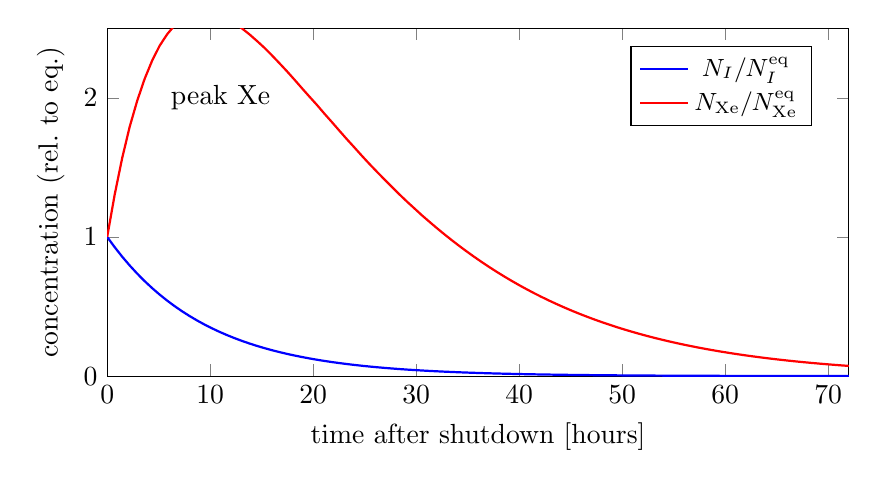
\begin{tikzpicture}
\begin{axis}[width=11cm,height=6cm,
   xlabel={time after shutdown [hours]},ylabel={concentration (rel.\ to eq.)},
   xmin=0,xmax=72,ymin=0,ymax=2.5,
   legend style={at={(0.95,0.95)},anchor=north east,font=\small}]
% N_I(t) = exp(-lambda_I t), lambda_I = ln 2/6.6 h = 0.105 /h
\addplot[domain=0:72,samples=100, thick, blue] {exp(-0.105*x)};
\addlegendentry{$N_I/N_I^\mathrm{eq}$}
% N_Xe(t) -- approximate; use lambda_Xe = ln 2 /9.2 = 0.0753/h, ratio lambda_I N_I^eq/(lambda_Xe N_Xe^eq) at saturation = ?
% In saturation N_Xe^eq ~ gamma_I Sigma_f /sigma_c, so lambda_I N_I^eq = gamma_I Sigma_f phi_n. lambda_Xe N_Xe^eq = lambda_Xe gamma_I Sigma_f /sigma_c. Ratio = phi_n sigma_c / lambda_Xe >> 1.
% Use ratio R = 5 for illustration
\addplot[domain=0:72,samples=100, thick, red] {exp(-0.0753*x) + 5*0.105/(0.0753-0.105)*(exp(-0.105*x)-exp(-0.0753*x))};
\addlegendentry{$N_\mathrm{Xe}/N_\mathrm{Xe}^\mathrm{eq}$}
\node at (axis cs:11,2.0) {peak Xe};
\end{axis}
\end{tikzpicture}
\end{center}

The Xe concentration peaks at $\sim 10$--$11$ hours after shutdown, possibly exceeding the operating equilibrium by a factor of $\sim 2$, then decays away with $t_{1/2}\sim 9$ h once the iodine source is exhausted.

\textbf{Restart danger.} If a restart is attempted during the Xe peak, the very high $^{135}$Xe concentration absorbs neutrons strongly (it is the strongest neutron poison known: $\sigma_c\sim 2.6\,\mathrm{Mb}$ at thermal). The reactor may fail to reach criticality, or the operator may withdraw control rods to compensate; once the Xe burns out (rapidly, due to $\sigma_c\phi_n\gg\lambda_\mathrm{Xe}$ as power rises), the reactivity surges. \textbf{This was the immediate trigger of the Chernobyl accident}: operators withdrew control rods to overcome xenon poisoning during a low-power test, and the subsequent xenon burnout caused a runaway reactivity excursion.

\textbf{Standard practice}: after shutdown, wait $\sim 24$--$48$ h for Xe to decay before restart; or operate continuously and avoid deep power transients.

\end{document}
